\documentclass[12pt, titlepage]{article}

\usepackage{pgfpages} 
\usepackage{booktabs}
\usepackage{tabularx}
\usepackage{hyperref}
\usepackage{outlines}
\usepackage{longtable}
\usepackage{enumitem,amssymb}
\usepackage{float}
\usepackage{adjustbox}
\usepackage{multirow}
\usepackage{ragged2e}
\newlist{todolist}{itemize}{2}
\setlist[todolist]{label=$\square$}
\hypersetup{
    colorlinks=true,
    citecolor=blue,
    filecolor=black,
    linkcolor=red,
    urlcolor=blue
}
\urlstyle{same}
\usepackage[round]{natbib}

%% Comments

\usepackage{color}

\newif\ifcomments\commentstrue %displays comments
%\newif\ifcomments\commentsfalse %so that comments do not display

\ifcomments
\newcommand{\authornote}[3]{\textcolor{#1}{[#3 ---#2]}}
\newcommand{\todo}[1]{\textcolor{red}{[TODO: #1]}}
\else
\newcommand{\authornote}[3]{}
\newcommand{\todo}[1]{}
\fi

\newcommand{\wss}[1]{\authornote{blue}{SS}{#1}} 
\newcommand{\plt}[1]{\authornote{magenta}{TPLT}{#1}} %For explanation of the template
\newcommand{\an}[1]{\authornote{cyan}{Author}{#1}}

%% Common Parts

\newcommand{\progname}{Software Engineering} % PUT YOUR PROGRAM NAME HERE
\newcommand{\authname}{Team 15, ASLingo
\\ Andrew Kil
\\ Cassidy Baldin
\\ Edward Zhuang
\\ Jeremy Langner
\\ Stanley Chan} % AUTHOR NAMES                  

\usepackage{hyperref}
    \hypersetup{colorlinks=true, linkcolor=blue, citecolor=blue, filecolor=blue,
                urlcolor=blue, unicode=false}
    \urlstyle{same}
                                


\begin{document}

\title{Verification and Validation Report: \progname} 
\author{\authname}
\date{\today}
	
\maketitle

\pagenumbering{roman}

\section{Revision History}

\begin{tabularx}{\textwidth}{p{3cm}p{3cm}X}
\toprule {\bf Date} & {\bf Contributors} & {\bf Notes}\\
\midrule
Feb 29, 2024 & Cassidy & Initial draft and formatting\\
Mar 4, 2024 & Andrew & Filled out table for learning progression\\
Mar 4, 2024 & Stanley & Added test results for performance requirements\\
Mar 4, 2024 & Cassidy & Added test results for tables 2,4,5 and 6\\
Mar 5, 2024 & Stanley & Added test to modules traceability matrix\\
Mar 6, 2024 & Andrew & Added automated testing information\\
Mar 6, 2024 & Cassidy & Added reflection, fixed table 6, added to automated testing section\\ 
Apr 4, 2024 & Jeremy and Cassidy & Updated system test results and tables according to VnVPlan\\ 
 &  & \\
\bottomrule
\end{tabularx}

~\newpage

\section{Symbols, Abbreviations and Acronyms}

\begin{longtable}{| c | p{7cm} |}
\caption{Naming Conventions and Terminology} \\
\hline
\textbf{Term, Abbreviation, or Acronym} & \textbf{Description}\\
\hline
A & Shorthand for Assumption\\
\hline
ASL & Shorthand for American Sign Language. It is a form of sign language primarily used in the US and in parts of Canada\\
\hline
ASLingo & The commercial name for the project\\
\hline
CV & Refers to Computer Vision, the field of technology that involves processing visual input to achieve various means.\\
\hline
CR & Shorthand for 'Cultural Requirements', a subsection of Non-Functional Requirements.\\
\hline
HSR & Shorthand for 'Health and Safety Requirements', a subsection of Non-Functional Requirements.\\
\hline
FR & Shorthand for Functional Requirements\\
\hline
LR & Shorthand for 'Legal Requirements', a subsection of Non-Functional Requirements.\\
\hline
LFR & Shorthand for 'Look and Feel Requirements', a subsection of Non-Functional Requirements.\\
\hline
MSR & Shorthand for 'Maintainability and Support Requirements', a subsection of Non-Functional Requirements.\\
\hline
OER & Shorthand for 'Operational and Environmental Requirements', a subsection of Non-Functional Requirements.\\
\hline
OpenCV & Refers to the Open Computer Vision Library library available for free to developers in order to develop Computer Vision applications.\\
\hline
PR & Shorthand for 'Performance Requirements', a subsection of Non-Functional Requirements.\\
\hline
SR & Shorthand for 'Security Requirements', a subsection of Non-Functional Requirements.\\
\hline
UHR & Shorthand for 'Usability and Humanity Requirements', a subsection of Non-Functional Requirements.\\
\bottomrule
\end{longtable}

\newpage

\tableofcontents

\listoftables %if appropriate

% \listoffigures %if appropriate

\newpage

\pagenumbering{arabic}

\section{General Information}

\subsection{Summary}

As a machine learning-based image recognition web app, ASLingo has many areas to be tested. The overall software will be broken down into modules. There will be a front-end, a back-end, a database, and a machine learning model which all need to be separately tested, along with physical hardware and compatibility. This document serves as a report of the testing done to ensure that this system has been properly and thoroughly tested to meet the requirements set by the \href{https://github.com/stanreee/sign-language-learning/blob/main/docs/SRS/SRS.pdf}{Software Requirements Specification}.  

\subsection{Objectives}

This document aims to outline the testing plan for ASLingo in order to create a functional and reliable product for users that aligns with the specified requirements. The team seeks to build confidence in stakeholders and users that the software is correct and meets or exceeds the initial intended goals, resulting in an overall satisfactory user experience.

\subsection{Relevant Documentation} 

Below is a list of the relevant documentation referenced within the Verification and Validation Plan.\\

\noindent The \href{https://github.com/stanreee/sign-language-learning/blob/main/docs/DevelopmentPlan/DevelopmentPlan.pdf}{Development Plan} outlines the roles of each team member and the areas that each member will focus on. This breakdown of team responsibilities allows the team to assign testing roles accordingly. This document also contains the tools that the team plans on using for testing.\\

\noindent The \href{https://github.com/stanreee/sign-language-learning/blob/main/docs/VnVPlan/VnVPlan.pdf}{VnV Plan} outlines the testing plan for the system, as well as outlining the test cases that the team will perform to ensure the project has been properly and thoroughly tested. This document also contains the tools that the team plans on using for testing.\\

\noindent The \href{https://github.com/stanreee/sign-language-learning/blob/main/docs/SRS/SRS.pdf}{Software Requirements Specification} lists the functional and non-functional requirements which will aid in testing by formulating a testing plan to meet each requirement. Non-functional requirements should be tested such that the fit criteria are met.\\

\noindent The \href{https://github.com/stanreee/sign-language-learning/blob/main/docs/HazardAnalysis/HazardAnalysis.pdf}{Hazard Analysis} identifies failure modes to determine the implementation strategies to mitigate them. These will be used as a part of the testing plan to ensure that the failures are covered.\\

\noindent The \href{https://github.com/stanreee/sign-language-learning/blob/main/docs/Design/SoftArchitecture/MG.pdf}{Module Guide} divides the software into modules. The team will build the testing plan around the modules.\\

\noindent The \href{https://github.com/stanreee/sign-language-learning/blob/main/docs/Design/SoftDetailedDes/MIS.pdf}{Module Interface Specification} further decomposes the software's modules into specific access routines. The team will build the testing plan such that each function and routine works as intended.

\section{Functional Requirements Evaluation}

\subsection{System Tests for ASL Learning Progression}

Many of the learning progression tests are redundant, as the development team and some participating users tested multiple ASL signs using the applications `Quiz' and `Practice' sections. All letters of the alphabet were tested to ensure correctness of the system, and all quiz levels were tested to ensure their functionality. 

\begin{longtable}{|p{1cm}|p{2.25cm}|p{3cm}|p{3cm}|p{1.75cm}|p{1.25cm}|p{1cm}|}
  \caption{System Tests for ASL Learning Progression} \\
  \hline
  \textbf{Test ID} & \textbf{Description} & \textbf{Input} & \textbf{Expected Output} & \textbf{Actual Output} & \textbf{Result} & \textbf{Req ID}\\
  \hline
  FRT1-LP1 & User performs ASL signs & Alphabetical signs `a', `b', `c' & The letters `a', `b', `c' are correct from user & The letters `a', `b', `c' are shown by user & Pass & FR1, FR2, FR4\\
  \hline
  FRT1-LP2 & Complete quiz & User goes to quiz page & System starts diagnostic quiz until user completes it & Quiz is started and completed by user & Pass & FR5, FR6, FR7 \\
  \hline
  FRT1-LP3 & Get live feedback from user signs & User signs letter `a' & Systems outputs letter `A' & System shows user letter `A' & Pass & FR1, FR2, FR3 \\
  \bottomrule
  \end{longtable}

\subsection{System Tests for Web Application}
\begin{longtable}{|p{1cm}|p{2.5cm}|p{2cm}|p{2cm}|p{2cm}|p{1.5cm}|p{1cm}|}
\caption{System Tests for Web Application} \\
\hline
\textbf{Test ID} & \textbf{Description} & \textbf{Input} & \textbf{Expected Output} & \textbf{Actual Output} & \textbf{Result} & \textbf{Req ID}\\
\hline
FRT3-U1 & User can access the web application & User opens web browser with the ASLingo application & User is able to access all pages of the application & User is able to access all pages of the application & Pass & FR1 \\
\bottomrule
\end{longtable}

\subsection{System Tests for Hardware}
\begin{longtable}{|p{1cm}|p{2.5cm}|p{2cm}|p{2cm}|p{2cm}|p{1.5cm}|p{1cm}|}
\caption{System Tests for Hardware} \\
\hline
\textbf{Test ID} & \textbf{Description} & \textbf{Input} & \textbf{Expected Output} & \textbf{Actual Output} & \textbf{Result} & \textbf{Req ID}\\
\hline
FRT4-HW1 & User is able to access the web camera & User goes to quiz page and starts a quiz & System is able to recognize user signs from their camera & System is able to recognize user signs from their camera & Pass & FR1 \\
\hline
FRT4-HW2 & Monitor web camera usability & User goes to quiz page and starts a quiz & User is notified if their camera is not working correctly & User is notified if their camera is not working correctly & Pass & FR1 \\
\bottomrule
\end{longtable}

\newpage
\section{Nonfunctional Requirements Evaluation}

\subsection{System Tests for Usability}

We will be testing our usability requirements using a survey for a group of testers to fill out after using the application for 15 minutes. The group of users will have an interest in learning ASL, and will be willing to fill out this questionnaire to give some perspective on the usability of our application. The list of survey questions and the link to the survey can be found in the Appendix \ref{appen}.

\subsection{Usability Testing Results}

Results from the Usability Survey conducted in partnership with the McMaster Sign Language Club. Participants had a mid to low range of skill levels, aka our target demographic.

\vspace{0.5cm}
\centering
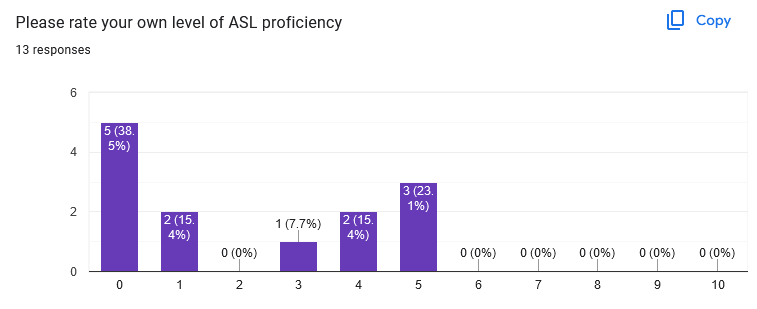
\includegraphics[scale=0.75]{Usability Survey Results/Q1.png}

\newpage

\vspace{0.5cm}
\centering
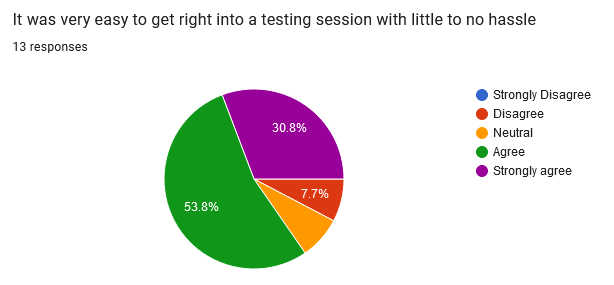
\includegraphics[scale=0.8]{Usability Survey Results/Q2.png}

\vspace{0.5cm}
\centering
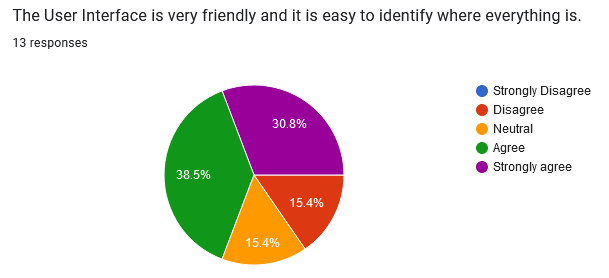
\includegraphics[scale=0.8]{Usability Survey Results/Q3.png}

\vspace{0.5cm}
\centering
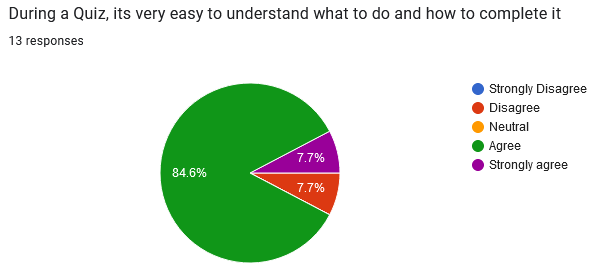
\includegraphics[scale=0.8]{Usability Survey Results/Q4.png}

\vspace{0.5cm}
\centering
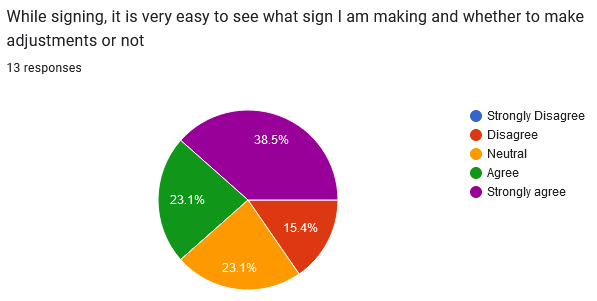
\includegraphics[scale=0.8]{Usability Survey Results/Q5.png}

\vspace{0.5cm}
\centering
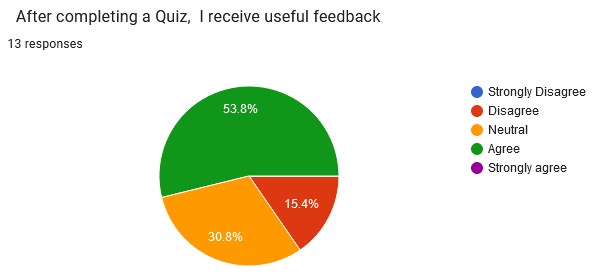
\includegraphics[scale=0.8]{Usability Survey Results/Q6.png}

\vspace{0.5cm}
\centering
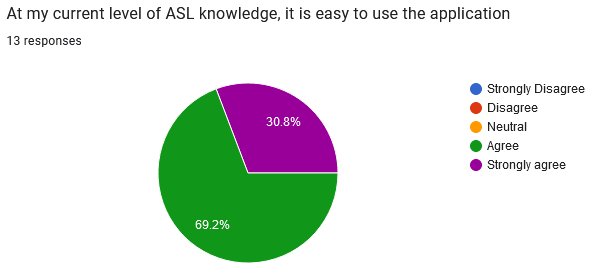
\includegraphics[scale=0.8]{Usability Survey Results/Q7.png}

\vspace{0.5cm}
\centering
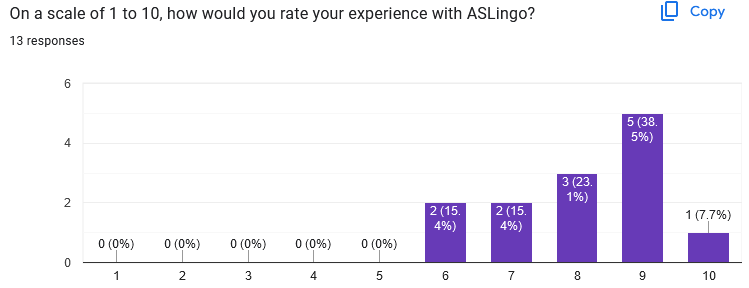
\includegraphics[scale=0.75]{Usability Survey Results/Q8.png}

\begin{longtable}{|p{1.5cm}|p{2.5cm}|p{2cm}|p{2cm}|p{2cm}|p{1.5cm}|p{1.5cm}|}
\caption{System Tests for Usability} \\
\hline
\textbf{Test ID} & \textbf{Description} & \textbf{Input} & \textbf{Expected Output} & \textbf{Actual Output} & \textbf{Result} & \textbf{Req ID}\\
\hline
NFRT1-UT1 & User is able to start application with no training & User opens web application & User is able to use application, completes question 2, 3 of survey with positive result & User is able to use application, results of question 2, 3 of survey sow most participants Agree or Strongly Agree & Pass & UHR1 \\
\hline
NFRT1-UT2 & User is able to complete a quiz with no training & User opens quiz page and starts a quiz & User is able to complete a quiz, completes question 4, 6 of survey with positive result & User is able to complete a quiz, results of question 4, 6 of survey sow most participants Agree or Strongly Agree & Pass & UHR1 \\
\hline
NFRT1-UT3 & User is able to use application with various hearing abilities & User opens application & User is able to use application, completes question 8 of survey with result over 75\% & User is able to use application, results of question 8 overall was 80\% from our user testing & Pass & UHR2 \\
\hline
NFRT1-UT4 & System should show user if input needs to be adjusted & User tries to complete quiz but their camera is not set up properly & System prompts user to fix camera settings & System prompts user to fix camera settings & Pass & UHR3 \\
\bottomrule
\end{longtable}



\RaggedRight
\subsection{System Tests for Performance}

\begin{longtable}{|p{1.5cm}|p{2.5cm}|p{2cm}|p{2cm}|p{2cm}|p{1.5cm}|p{1cm}|}
\caption{System Tests for Performance} \\
\hline
\textbf{Test ID} & \textbf{Description} & \textbf{Input} & \textbf{Expected Output} & \textbf{Actual Output} & \textbf{Result} & \textbf{Req ID}\\
\hline
NFRT2-PT1 & The application should respond to user input within 1 second. & The user should respond to the application's prompt. & The system should register the user's input and respond to the user quickly. & The system responded with the detected sign almost instantly. & Pass & PR1 \\
\hline
NFRT2-PT2 & The application should be able to accurately determine if the user has signed the correct response to the prompt 95\% of the time. & The user should sign in response to the application's prompt. & The application should register the user's signed input and determine if they have signed the required action correctly with 95\% overall accuracy. & Static hand signs are recognized with a total testing accuracy of around 98\%. Dynamic hand signs are very consistent, with the accuracy at around 94\%.  & Pass & PR2 \\
\bottomrule
\end{longtable}

\newpage
\section{Unit Testing}

\begin{longtable}{|p{1cm}|p{2.5cm}|p{2cm}|p{3cm}|p{3cm}|p{1cm}|p{1cm}|}
% \caption{System Tests for Hardware} \\
\hline
\textbf{Test ID} & \textbf{Description} & \textbf{Input} & \textbf{Expected Output} & \textbf{Actual Output} & \textbf{Result} & \textbf{Req ID}\\
\hline
DPM-UT1 & Tests the vector normalization function & [1.0, 2.0, 3.0, -4.0], [4.0, -6.0, 3.0, -1.0] & [0.25, 0.5, 0.75, -1], [4.0/6.0, -6.0/6.0, 3.0/6.0, -1.0/6.0] & [0.25, 0.5, 0.75, -1], [4.0/6.0, -6.0/6.0, 3.0/6.0, -1.0/6.0] & Pass & FR2 \\
\hline
DPM-UT2 & Tests the feature processing function & [[1.0, 2.0, 5.0], [3.0, 4.0, -2.0], [5.0, 6.0, -3.0]], [[-1.0, 1.0, 0.0], [2.0, 1.0, -3.0], [-3.0, 2.0, 1.0]] & [[0.0, 0.0, -2.0], [-2.0, -2.0, 5.0], [-4.0, -4.0, 6.0]], [[0.0, 0.0, 0.0], [-3.0, 0.0, 3.0], [2.0, -1.0, -1.0]] & Correct & Pass & FR2 \\
\bottomrule
\end{longtable}


\section{Changes Due to Testing}

% \wss{This section should highlight how feedback from the users and from 
% the supervisor (when one exists) shaped the final product.  In particular 
% the feedback from the Rev 0 demo to the supervisor (or to potential users) 
% should be highlighted.}
\begin{itemize}

    \item A change due to testing involves ensuring efficiency of sign recognition is held to a high standard from NFRT2 which outlines having a 95\% accuracy of determining the user's hand sign.

    \item From our user testing, we also want to ensure that new and existing users of our application can get the best learning experience possible through a responsive, well designed and tested application. Before, the layout of our application was what seemed natural for us, but as we gathered usability testing data from end users we realized we had to make changes to the user interface.
\end{itemize}

\section{Automated Testing}

Automated testing is taken care of by the automatic linter flake8 upon every push to the repository to ensure that our python code is in line with the styling guide of flake8. We are also using a local and automatic linter eslint for our Javascript code for the front end of our application. 

\section{Trace to Requirements}

\paragraph{Functional Requirements to System Tests}
\begin{table}[ht]
\centering
\resizebox{\textwidth}{!}{
\begin{tabular}{llllllllllllll}
                                 & \multicolumn{7}{c}{FR Req.}                                                                                                                                                                                                                                                                                                           \\ \cline{2-8} 
\multicolumn{1}{l|}{System Test} & \multicolumn{1}{l|}{1} & \multicolumn{1}{l|}{2} & \multicolumn{1}{l|}{3} & \multicolumn{1}{l|}{4} & \multicolumn{1}{l|}{5} & \multicolumn{1}{l|}{6} & \multicolumn{1}{l|}{7}  \\ \hline

\multicolumn{1}{|l|}{FRT1-LP1}   & \multicolumn{1}{l|}{X}  & \multicolumn{1}{l|}{X} & \multicolumn{1}{l|}{}  & \multicolumn{1}{l|}{X}  & \multicolumn{1}{l|}{}  & \multicolumn{1}{l|}{}  & \multicolumn{1}{l|}{}    \\ \hline

\multicolumn{1}{|l|}{FRT1-LP2}   & \multicolumn{1}{l|}{}  & \multicolumn{1}{l|}{}  & \multicolumn{1}{l|}{}  & \multicolumn{1}{l|}{}  & \multicolumn{1}{l|}{X}  & \multicolumn{1}{l|}{X} & \multicolumn{1}{l|}{X}    \\ \hline

\multicolumn{1}{|l|}{FRT1-LP3}   & \multicolumn{1}{l|}{X}  & \multicolumn{1}{l|}{X}  & \multicolumn{1}{l|}{X}  & \multicolumn{1}{l|}{}  & \multicolumn{1}{l|}{}  & \multicolumn{1}{l|}{}  & \multicolumn{1}{l|}{}   \\ \hline

\multicolumn{1}{|l|}{FRT2-U1}    & \multicolumn{1}{l|}{X}  & \multicolumn{1}{l|}{}  & \multicolumn{1}{l|}{}  & \multicolumn{1}{l|}{}  & \multicolumn{1}{l|}{}  & \multicolumn{1}{l|}{}  & \multicolumn{1}{l|}{}     \\ \hline

\multicolumn{1}{|l|}{FRT3-HW1}   & \multicolumn{1}{l|}{X} & \multicolumn{1}{l|}{}  & \multicolumn{1}{l|}{}  & \multicolumn{1}{l|}{}  & \multicolumn{1}{l|}{}  & \multicolumn{1}{l|}{}    & \multicolumn{1}{l|}{}   \\ \hline

\multicolumn{1}{|l|}{FRT3-HW2}   & \multicolumn{1}{l|}{X}  & \multicolumn{1}{l|}{}  & \multicolumn{1}{l|}{}  & \multicolumn{1}{l|}{}  & \multicolumn{1}{l|}{}  & \multicolumn{1}{l|}{}  & \multicolumn{1}{l|}{}    \\ \hline
\end{tabular}}
\end{table}

\paragraph{Non Functional Requirements to System Tests}

\begin{table}[H]
\centering
\resizebox{\textwidth}{!}{
\begin{tabular}{lllllll}
                                 & \multicolumn{3}{c}{UHR}                                                  & \multicolumn{2}{c}{PR}                                                   \\ \cline{2-6} 
\multicolumn{1}{l|}{System Test} & \multicolumn{1}{l|}{1} & \multicolumn{1}{l|}{2} & \multicolumn{1}{l|}{3} & \multicolumn{1}{l|}{1} & \multicolumn{1}{l|}{2} \\ \hline
\multicolumn{1}{|l|}{NFRT1-UT1}  & \multicolumn{1}{l|}{X} & \multicolumn{1}{l|}{}  & \multicolumn{1}{l|}{}  & \multicolumn{1}{l|}{}  & \multicolumn{1}{l|}{}   \\ \hline
\multicolumn{1}{|l|}{NFRT1-UT2}  & \multicolumn{1}{l|}{X} & \multicolumn{1}{l|}{}  & \multicolumn{1}{l|}{}  & \multicolumn{1}{l|}{}  & \multicolumn{1}{l|}{}   \\ \hline
\multicolumn{1}{|l|}{NFRT1-UT3}  & \multicolumn{1}{l|}{}  & \multicolumn{1}{l|}{X} & \multicolumn{1}{l|}{}  & \multicolumn{1}{l|}{}  & \multicolumn{1}{l|}{}    \\ \hline
\multicolumn{1}{|l|}{NFRT1-UT4}  & \multicolumn{1}{l|}{}  & \multicolumn{1}{l|}{}  & \multicolumn{1}{l|}{X} & \multicolumn{1}{l|}{}  & \multicolumn{1}{l|}{}   \\ \hline
\multicolumn{1}{|l|}{NFRT2-PT1}  & \multicolumn{1}{l|}{}  & \multicolumn{1}{l|}{}  & \multicolumn{1}{l|}{}  & \multicolumn{1}{l|}{X} & \multicolumn{1}{l|}{}   \\ \hline
\multicolumn{1}{|l|}{NFRT2-PT2}  & \multicolumn{1}{l|}{}  & \multicolumn{1}{l|}{}  & \multicolumn{1}{l|}{}  & \multicolumn{1}{l|}{}  & \multicolumn{1}{l|}{X}  \\ \hline
\end{tabular}
}
\end{table}
		
\section{Trace to Modules}

\paragraph{System Tests to Modules}
\begin{table}[ht]
\centering
\resizebox{\textwidth}{!}{
\begin{tabular}{lllllllllllll}
                                 & \multicolumn{12}{c}{Module}                                                                                                                                                                                                                                                                                                           \\ \cline{2-13} 
\multicolumn{1}{l|}{System Test} & \multicolumn{1}{l|}{M1} & \multicolumn{1}{l|}{M2} & \multicolumn{1}{l|}{M3} & \multicolumn{1}{l|}{M4} & \multicolumn{1}{l|}{M5} & \multicolumn{1}{l|}{M6} & \multicolumn{1}{l|}{M7} & \multicolumn{1}{l|}{M8} & \multicolumn{1}{l|}{M9} & \multicolumn{1}{l|}{M10} & \multicolumn{1}{l|}{M11} & \multicolumn{1}{l|}{M12} \\ \hline
\multicolumn{1}{|l|}{FRT2-LP1}   & \multicolumn{1}{l|}{X}  & \multicolumn{1}{l|}{X}  & \multicolumn{1}{l|}{}  & \multicolumn{1}{l|}{}  & \multicolumn{1}{l|}{}  & \multicolumn{1}{l|}{}  & \multicolumn{1}{l|}{}  & \multicolumn{1}{l|}{X}  & \multicolumn{1}{l|}{}  & \multicolumn{1}{l|}{}   & \multicolumn{1}{l|}{}  & \multicolumn{1}{l|}{}      \\ \hline
\multicolumn{1}{|l|}{FRT2-LP2}   & \multicolumn{1}{l|}{X}  & \multicolumn{1}{l|}{}  & \multicolumn{1}{l|}{}  & \multicolumn{1}{l|}{}  & \multicolumn{1}{l|}{}  & \multicolumn{1}{l|}{}  & \multicolumn{1}{l|}{}  & \multicolumn{1}{l|}{X}  & \multicolumn{1}{l|}{X}  & \multicolumn{1}{l|}{}   & \multicolumn{1}{l|}{X}  & \multicolumn{1}{l|}{}     \\ \hline
\multicolumn{1}{|l|}{FRT2-LP3}   & \multicolumn{1}{l|}{X}  & \multicolumn{1}{l|}{X}  & \multicolumn{1}{l|}{X}  & \multicolumn{1}{l|}{}  & \multicolumn{1}{l|}{}  & \multicolumn{1}{l|}{}  & \multicolumn{1}{l|}{}  & \multicolumn{1}{l|}{X}  & \multicolumn{1}{l|}{}  & \multicolumn{1}{l|}{X}   & \multicolumn{1}{l|}{}  & \multicolumn{1}{l|}{}      \\ \hline
\multicolumn{1}{|l|}{FRT3-U1}    & \multicolumn{1}{l|}{}  & \multicolumn{1}{l|}{}  & \multicolumn{1}{l|}{}  & \multicolumn{1}{l|}{}  & \multicolumn{1}{l|}{}  & \multicolumn{1}{l|}{}  & \multicolumn{1}{l|}{}  & \multicolumn{1}{l|}{X}  & \multicolumn{1}{l|}{}  & \multicolumn{1}{l|}{}   & \multicolumn{1}{l|}{}  & \multicolumn{1}{l|}{}      \\ \hline
\multicolumn{1}{|l|}{FRT4-HW1}   & \multicolumn{1}{l|}{}  & \multicolumn{1}{l|}{}  & \multicolumn{1}{l|}{}  & \multicolumn{1}{l|}{}  & \multicolumn{1}{l|}{}  & \multicolumn{1}{l|}{}  & \multicolumn{1}{l|}{}  & \multicolumn{1}{l|}{X}  & \multicolumn{1}{l|}{}  & \multicolumn{1}{l|}{}   & \multicolumn{1}{l|}{}  & \multicolumn{1}{l|}{}      \\ \hline
\multicolumn{1}{|l|}{FRT4-HW2}   & \multicolumn{1}{l|}{}  & \multicolumn{1}{l|}{}  & \multicolumn{1}{l|}{}  & \multicolumn{1}{l|}{}  & \multicolumn{1}{l|}{}  & \multicolumn{1}{l|}{}  & \multicolumn{1}{l|}{}  & \multicolumn{1}{l|}{X}  & \multicolumn{1}{l|}{}  & \multicolumn{1}{l|}{}   & \multicolumn{1}{l|}{}  & \multicolumn{1}{l|}{}      \\ \hline
\multicolumn{1}{|l|}{NFRT1-UT1}   & \multicolumn{1}{l|}{}  & \multicolumn{1}{l|}{}  & \multicolumn{1}{l|}{}  & \multicolumn{1}{l|}{}  & \multicolumn{1}{l|}{}  & \multicolumn{1}{l|}{}  & \multicolumn{1}{l|}{}  & \multicolumn{1}{l|}{}  & \multicolumn{1}{l|}{X}  & \multicolumn{1}{l|}{}   & \multicolumn{1}{l|}{}  & \multicolumn{1}{l|}{}      \\ \hline
\multicolumn{1}{|l|}{NFRT1-UT2}   & \multicolumn{1}{l|}{}  & \multicolumn{1}{l|}{}  & \multicolumn{1}{l|}{}  & \multicolumn{1}{l|}{}  & \multicolumn{1}{l|}{}  & \multicolumn{1}{l|}{}  & \multicolumn{1}{l|}{}  & \multicolumn{1}{l|}{}  & \multicolumn{1}{l|}{X}  & \multicolumn{1}{l|}{}   & \multicolumn{1}{l|}{}  & \multicolumn{1}{l|}{}      \\ \hline
\multicolumn{1}{|l|}{NFRT1-UT3}   & \multicolumn{1}{l|}{}  & \multicolumn{1}{l|}{}  & \multicolumn{1}{l|}{}  & \multicolumn{1}{l|}{}  & \multicolumn{1}{l|}{}  & \multicolumn{1}{l|}{}  & \multicolumn{1}{l|}{}  & \multicolumn{1}{l|}{}  & \multicolumn{1}{l|}{X}  & \multicolumn{1}{l|}{}   & \multicolumn{1}{l|}{}  & \multicolumn{1}{l|}{}     \\ \hline
\multicolumn{1}{|l|}{NFRT1-UT4}   & \multicolumn{1}{l|}{X}  & \multicolumn{1}{l|}{}  & \multicolumn{1}{l|}{}  & \multicolumn{1}{l|}{}  & \multicolumn{1}{l|}{}  & \multicolumn{1}{l|}{}  & \multicolumn{1}{l|}{}  & \multicolumn{1}{l|}{X}  & \multicolumn{1}{l|}{}  & \multicolumn{1}{l|}{}   & \multicolumn{1}{l|}{}  & \multicolumn{1}{l|}{}      \\ \hline
\multicolumn{1}{|l|}{NFRT2-PT1}   & \multicolumn{1}{l|}{}  & \multicolumn{1}{l|}{}  & \multicolumn{1}{l|}{X}  & \multicolumn{1}{l|}{}  & \multicolumn{1}{l|}{X}  & \multicolumn{1}{l|}{}  & \multicolumn{1}{l|}{}  & \multicolumn{1}{l|}{}  & \multicolumn{1}{l|}{}  & \multicolumn{1}{l|}{}   & \multicolumn{1}{l|}{}  & \multicolumn{1}{l|}{}      \\ \hline
\multicolumn{1}{|l|}{NFRT2-PT2}   & \multicolumn{1}{l|}{X}  & \multicolumn{1}{l|}{X}  & \multicolumn{1}{l|}{}  & \multicolumn{1}{l|}{}  & \multicolumn{1}{l|}{}  & \multicolumn{1}{l|}{}  & \multicolumn{1}{l|}{X}  & \multicolumn{1}{l|}{}  & \multicolumn{1}{l|}{}  & \multicolumn{1}{l|}{}   & \multicolumn{1}{l|}{}  & \multicolumn{1}{l|}{}      \\ \hline
\end{tabular}}
\end{table}

% \bibliographystyle{plainnat}
% \bibliography{../../refs/References}

\newpage{}

\section{Appendix}

\subsection{Usability Survey Questions} \label{appen}

A link to the survey that participants will be given can be found \href{https://docs.google.com/forms/d/e/1FAIpQLSelcMIJ-egkwLc7gO8MhqO35-FpTtQ6efCKnogOOKVVsrdWNA/viewform}{here}. Participants will be asked to rank how they felt about the following statements, with the response options being Strongly Disagree, Disagree, Neutral, Agree, and Strongly Agree.

\begin{enumerate}

\item Please rate your own level of ASL proficiency on a scale of 1-10 \newline [ 1 = I know absolutely nothing, 10 = I sign at a high level]
\item From Strongly Disagree to Strongly Aggree, rate the following sentence: It was very easy to get right into a testing session with little to no hassle
\item From Strongly Disagree to Strongly Aggree, rate the following sentence: The User Interface is very friendly and it is easy to identify where everything is
\item From Strongly Disagree to Strongly Aggree, rate the following sentence: During a Quiz, its very easy to understand what to do and how to complete it
\item From Strongly Disagree to Strongly Aggree, rate the following sentence: While signing, it is very easy to see what sign I am making and whether to make adjustments or not
\item From Strongly Disagree to Strongly Aggree, rate the following sentence:  After completing a Quiz,  I receive useful feedback
\item From Strongly Disagree to Strongly Aggree, rate the following sentence: At my current level of ASL knowledge, it is easy to use the application
\item How would you rate your overall experience with ASLingo on a scale of 1-10 \newline [ 1 = Terrible, 10 = Fantastic]
\end{enumerate}

\subsection{Appendix --- Reflection}

The information in this section will be used to evaluate the team members on the
graduate attribute of Reflection.  Please answer the following question:

\begin{enumerate}
  \item In what ways was the Verification and Validation (VnV) Plan different
  from the activities that were actually conducted for VnV?  If there were
  differences, what changes required the modification in the plan?  Why did
  these changes occur?  Would you be able to anticipate these changes in future
  projects?  If there weren't any differences, how was your team able to clearly
  predict a feasible amount of effort and the right tasks needed to build the
  evidence that demonstrates the required quality?  (It is expected that most
  teams will have had to deviate from their original VnV Plan.)
\end{enumerate}

The Verification and Validation (VnV) plan is different than the tests that were actually conducted for the VnV Report in many ways. One main difference was that our team wrote more tests than the tests that were in the original VnV plan, and we also performed even more tests than the ones that were written. This is because when we wrote the VnV plan in November, we only had the proof of concept version of our project completed, so the tests that were written were for an earlier version of the project, or an ideal version of our project. While working on the project for our Rev0 demo, the team was constantly testing both the front and back end to ensure that the required functionality was working according to the specifications lead out in the SRS document. This testing was in line with some of the new test cases that were added to the VnV plan, but many were redundant and are not shown in the final report or plan (such as testing each letter of the alphabet individually multiple times with different people and in different environments) to reduce the length of the report. We think that some of these changes could be anticipated in future projects if a lot more time was given to all the intricacies of what the final project would look and perform like, but some changes to things like the usability of the project you can only really know after doing testing with users and other stakeholders and are harder to predict from a glance. 

\end{document}